\documentclass[../main.tex]{subfiles}
%!TEX root = ./analysisThrusterAssemblySelection.tex
\graphicspath {{../}}

\begin{document}
\subsection{Motor and Propeller Selection} \label{motorSelect}

\begin{figure}[H]
	\centering
	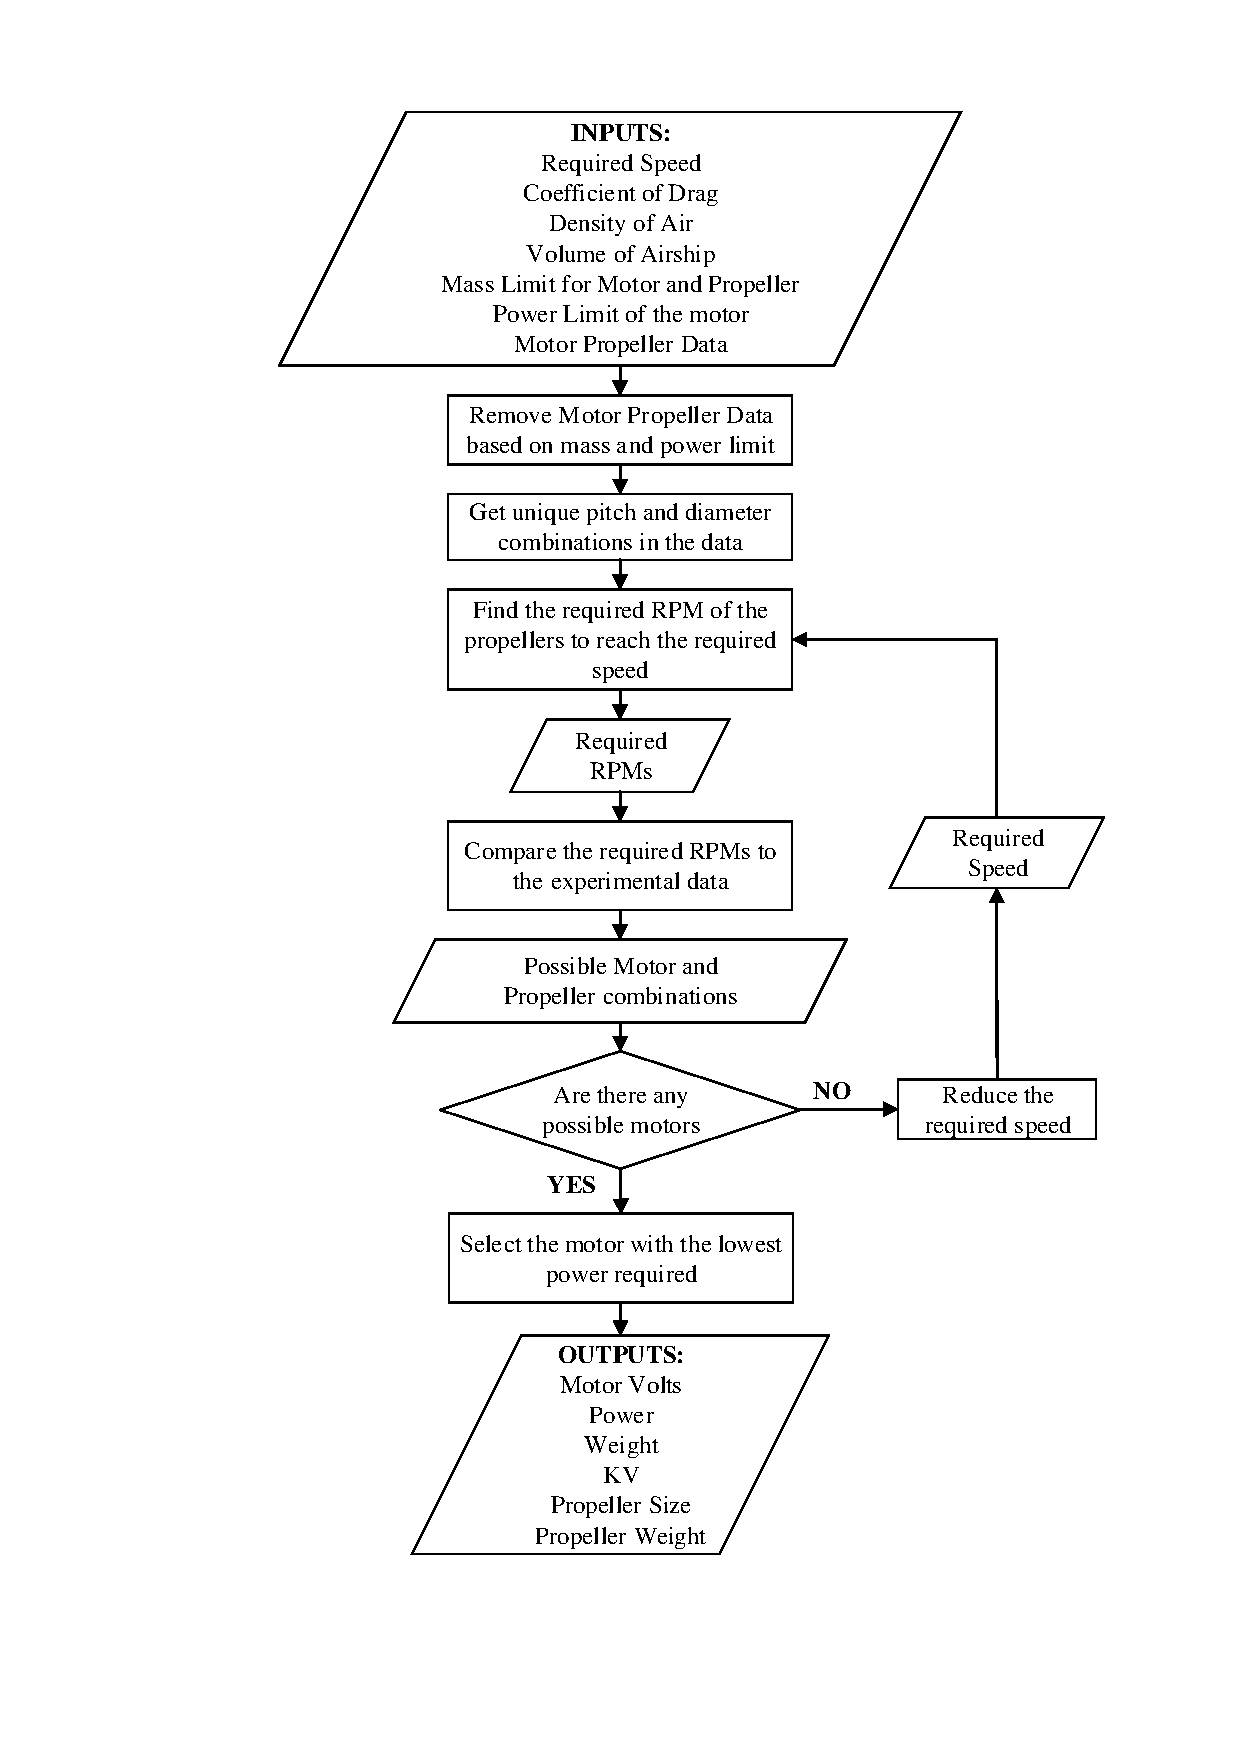
\includegraphics[width=0.7\linewidth]{img/paramaterization/motorPropellerChoice.pdf}
	\caption{Parametrization Outline For Motor and Propeller Selection}
	\label{fig:motorOutline}
\end{figure}

The selection of the motor and propeller relies on experimental data. This was sourced from Fly Brushless \cite{propMotData} and the data is used to get realistic values based on the required speed. To narrow the selection of data propellers were only chosen from APC, since there was many different sizes on large amounts of data on them on Fly Brushless. Roughly 2000 points of data was collected, this was reduced to 60 in order to improve computation time and since most of the others would never be chosen by the program.\\

The selection works by first filtering the experimental data to get motors that fit within the power limit set by the program. From this the unique pitch and diameter combinations are analysed to find their required rotational speed to meet the required speed. The required rotational speed is found iteratively, increasing each time until the thrust curve intersects the drag curve above the required speed. The analysis for the thrust calculation is found in Appendix \ref{appendix:thrust} and the drag analysis is found in Appendix \ref{appendix:drag}. To increase the rotational speed guess of each iteration an equation is used to approximate it based on the zero thrust speed. The equation relates the maximum RPM ($nm$) to the zero thrust speed $V_{zero}$, pitch $P$ and diameter of propeller $D$:

\begin{equation}
nm = \frac{V_{}zero}{0.2D+0.74P}
\end{equation}

For each iteration the speed is increased by $1m/s$ scaling the RPM proportional until the required speed is met. These results are then compared to the experimental data and the data point which requires the lowest power is selected. If there is no matching experimental data the program is looped with a lower required speed. The code for this selection can be seen in Section \ref{code:motorSelect}

\subsection{Battery Selection} \label{batterySelect}

\begin{figure}[H]
	\centering
	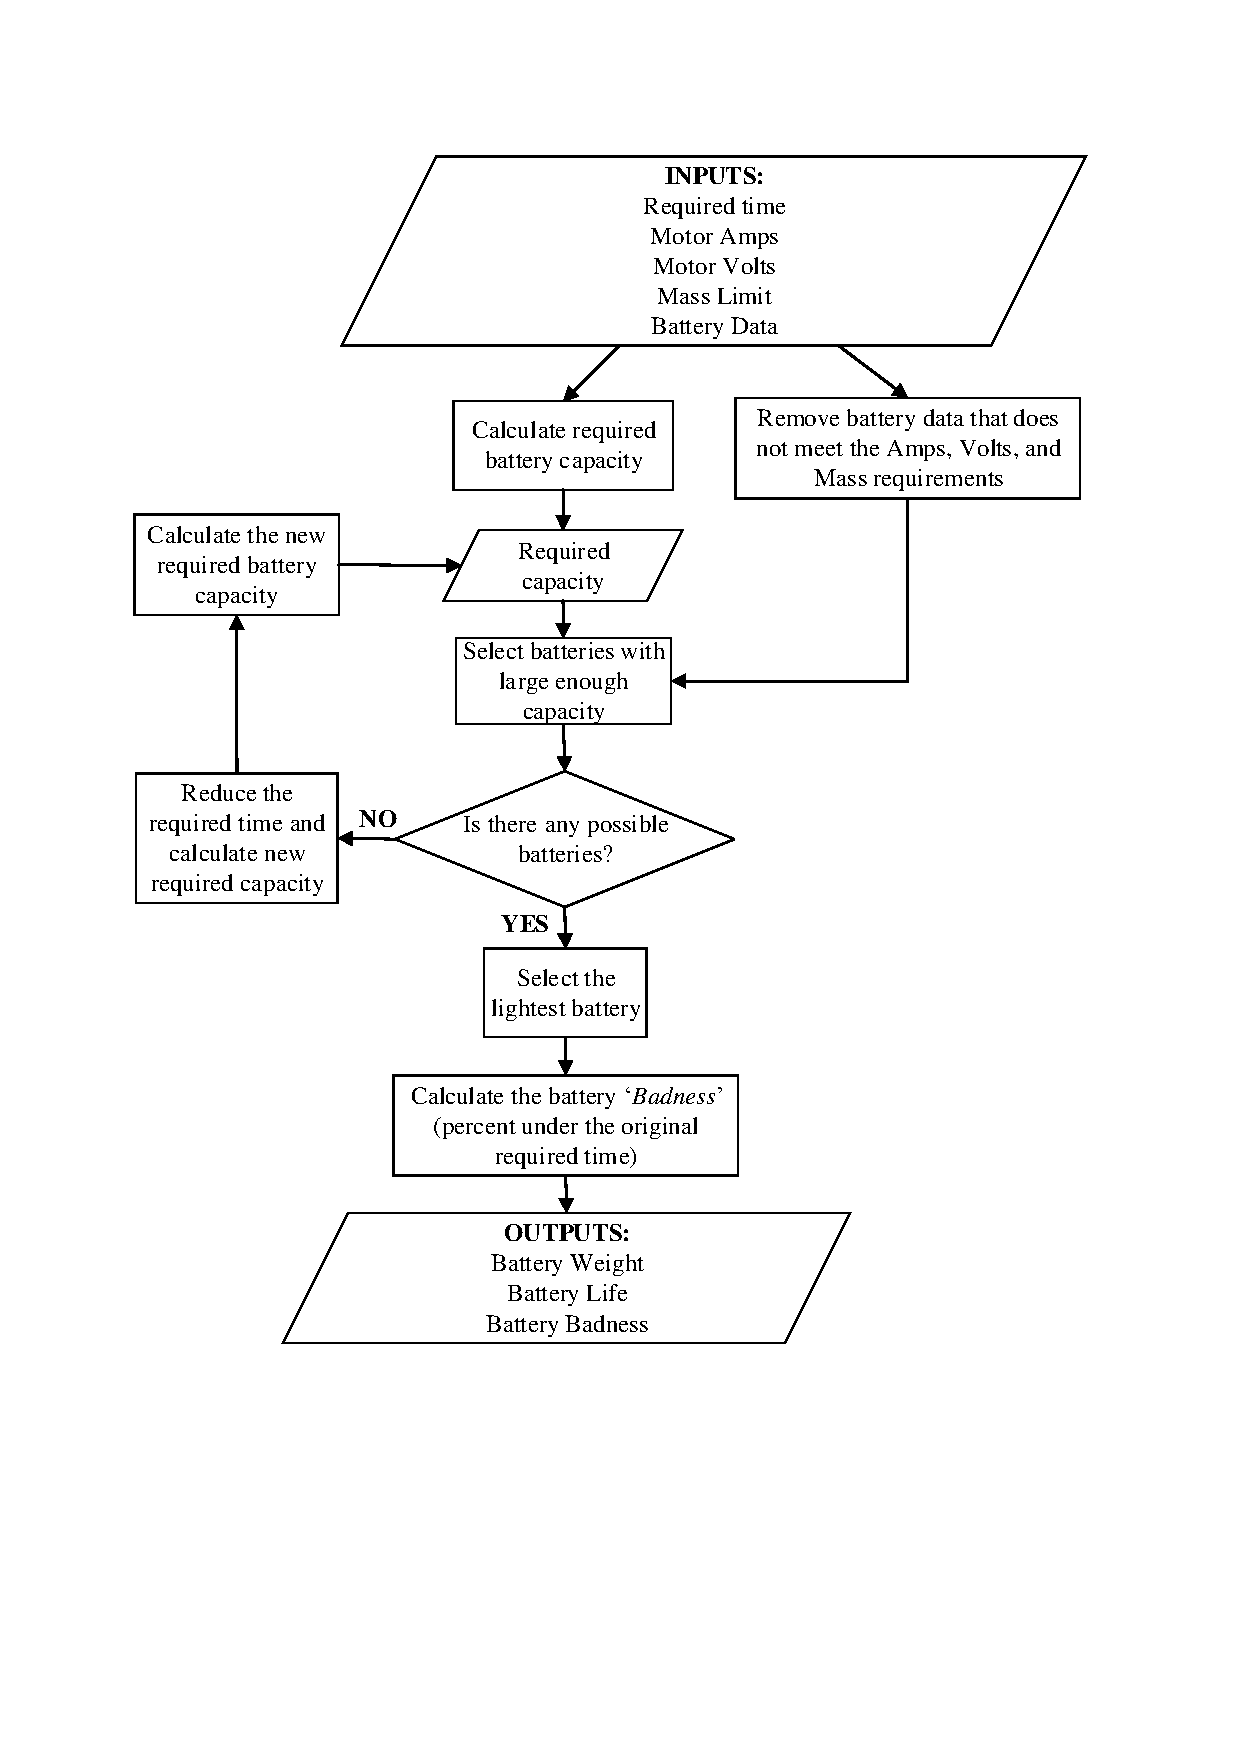
\includegraphics[width=0.95\linewidth]{img/paramaterization/batteryChoice.pdf}
	\caption{Parametrization Outline For Battery Selection}
	\label{fig:batteryOutline}
\end{figure}

The battery selection follows the propeller and motor selection since a required input is the power usage of the motor. Similar to the motor and propeller, the battery selection relies on real battery data to get weights and dimensions of batteries. This data was taken from Hobby King \cite{Hobbyking} using the Lipo Search. Many different capacities were chosen with different number of cells to accommodate the different motor sizes and varying required flight times.\\

The data is first filtered to remove batteries that are too heavy, don't have enough discharge, and/or don't have the required voltage. Using the inputs to the function the required carrying capacity is calculated. This is done using Equation \ref{eqn:battCap}, where capacity is in $mAh$, motor amperage ($A$) is in amps, and time ($t$) is in hours.

\begin{equation} \label{eqn:battCap}
\text{Capacity} = At*1000;
\end{equation}

This calculated value is then compared to the data and the lightest matching battery is picked. If no batteries meet the requirements the required time is reduced and the capacity is recalculated until it matches a battery. The chosen battery information is used to get the weight of the thruster assembly and parametrise the battery enclosure. The code for this can be seen in Section \ref{code:batterySelect}.

\end{document}